% brief.tex -- supervisor brief: what we built, what we found, what is wrong.
% Build: cd paper && pdflatex -interaction=nonstopmode brief && pdflatex -interaction=nonstopmode brief
% Body: brief_body.tex (sections 1-8); issue boxes: brief_issues.tex (input from section 6 of the body).
% Figures are read from figs/ relative to this folder.
\documentclass[11pt,a4paper]{article}
\usepackage[margin=2cm]{geometry}
\usepackage[T1]{fontenc}
\usepackage[utf8]{inputenc}
\usepackage{lmodern}
\usepackage{booktabs}
\usepackage{array}
\usepackage{graphicx}
\usepackage{float}
\usepackage{capt-of}
\usepackage{amsmath,amssymb}
\usepackage{enumitem}
\setlist{topsep=2pt,itemsep=1pt,parsep=0pt,partopsep=0pt,leftmargin=*}
\usepackage{parskip}
\setlength{\parskip}{3pt plus 1pt}
\usepackage{xcolor}
\usepackage[hidelinks]{hyperref}

% Ragged-right paragraph column (no inter-word stretching in narrow cells).
\newcolumntype{L}[1]{>{\raggedright\arraybackslash}p{#1}}

\newenvironment{issuebox}[1]{\par\medskip\noindent\textbf{#1}\par\nopagebreak\small}{\par\medskip}
\newenvironment{notebox}[1]{\par\medskip\noindent\textbf{#1}\par\nopagebreak\small}{\par\medskip}

\newcommand{\takeaway}[1]{\par\noindent\textbf{Takeaway: }#1\par}

% Title, author and date are typeset by hand (compact block) below.
\title{E-bike battery swapping in NYC: what we built, what we found, what is wrong}
\author{Mingchen Yuan}
\date{14 October 2026}

\begin{document}
\begin{center}
{\Large\bfseries E-bike battery swapping in NYC:\\[2pt] what we built, what we found, what is wrong\par}\vspace{2pt}
{\normalsize Mingchen Yuan \quad\textperiodcentered\quad 14 October 2026\par}
\end{center}
\vspace{-6pt}
% brief_body.tex -- sections only; the assembler supplies the preamble
% (booktabs, array, graphicx, hyperref). Figures are read from figs/
% relative to paper/ (the absolute path contains a space, which graphicx
% does not accept reliably).
%
% Sources of every number (cited again next to each table):
%   README  = OR Model-Battery Swap/README.md (sections 5-7)
%   E2U     = ebike_swap_sim/outputs/e2u_round3/RESULTS_final.md
%   E3U     = ebike_swap_sim/outputs/e3u_round3/RESULTS_final.md
%   E4U     = ebike_swap_sim/outputs/e4u_round3/RESULTS_final.md
%   E8      = ebike_swap_sim/outputs/e8_round3/RESULTS_final.md
%   E1      = ebike_swap_sim/outputs/e1/RESULTS.md
%   REVIEW  = notes/E2_formulation_review.md
%   COST    = notes/cost_calibration.md (section 9) and notes/DECISIONS.md (R2.1)
%   SUMMARY = notes/SUMMARY.md (round headers carry the dates)
%
% Vocabulary (used everywhere in this brief): "plan" = the E2 integer program,
% "rule" = the nearest-rider baseline policy, costs in USD after the number,
% "dropped" = unserved order.

\ifdefined\takeaway\else
\newcommand{\takeaway}[1]{\par\noindent\textbf{Takeaway: }#1\par}
\fi
\newcommand{\caveat}[1]{\par\noindent\emph{Caveat: }#1\par}

% ======================================================================
\section*{1. One-page summary}
% ======================================================================

\noindent\textbf{The question.} Does a coordinated plan (the supervisor's integer program E2: who delivers what, when to swap, when to charge, when to ship batteries) beat a simple dispatch rule on the same evening? And do stations, spare batteries and shuttles matter?

\noindent\textbf{What we built.}
\begin{itemize}\small\setlength{\itemsep}{0pt}
  \item E2 implemented as written (equations (1)--(33), Gurobi); toy example reproduced exactly ($J = 12.5$).
  \item A comparable baseline rule: nearest free rider, swap at 3 of 12 levels, charge on demand, no crystal ball.
  \item Instance generator with USD costs from NYC sources and a literature-based demand model; one independent cost checker prices both methods.
  \item NYC data pipeline (real Midtown restaurants, census weights, real candidate sites); three experiment rounds, 10 seeds, every solver cell filled.
\end{itemize}

\noindent\textbf{Headline results} (final, round 3; gap $=$ (rule $-$ plan)/rule; $\pm$ is a 95\,\% $t$-interval over random evenings).
% source: README section 6.1; E2U summary; E3U summary; E4U summary; E8 section 2
\begin{center}\small
\begin{tabular}{@{}L{3.0cm}L{8.2cm}L{3.7cm}@{}}
\toprule
Question & Result & Read \\
\midrule
Value of coordination & \textbf{29.6\,\% $\pm$ 5.6} cheaper, cheaper on all 30 evenings; 15.4 / 31.2 / 42.1\,\% at quiet / normal / busy demand & Sec.\ 5, E2u \\
Where the saving is & 59\,\% lateness, 32\,\% customer waiting, 8\,\% dropped orders, $<1$\,\% riding $+$ electricity & Sec.\ 5, E2u \\
A 90\,\% service guarantee & costs 0.2\,\% at quiet and 5.5\,\% at normal demand; \textbf{impossible} at 1.5$\times$ demand with 6 bikes & Sec.\ 5, service share \\
Shuttles and stations & shuttles worth $\approx 0$ (8.6 USD, and only because of end-of-day battery targets); 1 spare battery per site is enough for the plan & Sec.\ 5, E3u / E4u \\
Real Midtown data & \textbf{31.8\,\% $\pm$ 8.2} (busiest-cell sites), 30.5\,\% $\pm$ 8.6 (landmark sites); positive on 20 of 20 & Sec.\ 5, E8 \\
Where to put stations & \textbf{one} co-located site (L02, NoMad) with 3--4 spares and 2 chargers at every budget; 654 USD per evening, 85.2\,\% served; a second site never pays & Sec.\ 5, E9 \\
\bottomrule
\end{tabular}
\end{center}

% Numbering below matches Section 6 (Issues 1, 2, 3 and 5).
\par\smallskip\noindent\textbf{Problems found (numbers as in Section 6)}\par
\begin{itemize}\small\setlength{\itemsep}{0pt}
  \item \textbf{Issue 1 -- The 29.6\,\% mixes coordination with perfect foresight.} The plan sees all orders at 17:00; the rule learns them as they arrive. Rolling-horizon test pending.
  \item \textbf{Issue 2 -- Stations and chargers never bind at this scale.} 9 spares for 6 bikes over 4 h: chargers and power are worth 0 USD, the relaxed plan buys 0 kWh in 20 of 20 Midtown runs, moving the sites changes the plan's cost by $\le 0.41$ USD. Same on the siting family (Issue 13).
  \item \textbf{Issue 3 -- Shuttle value exists only because of the end-of-day battery targets.} 8.6 USD with the targets, 0.00 USD without, on 15 of 15 layout--seed pairs.
  \item \textbf{Issue 5 -- The wage convention decides whether the plan drops orders.} With rider wages priced per order (\texttt{usd\_A}) the plan drops 83--86\,\% of orders; we use \texttt{usd\_sunk} (wages sunk), a modelling decision, not a fact.
\end{itemize}
\par\smallskip

\noindent\textbf{Decisions needed from the supervisor} (details: Issues 3, 4, 5; next steps in Section 7).
\begin{enumerate}\small\setlength{\itemsep}{0pt}
  \item \textbf{End-of-day battery targets:} keep as written (0.3 USD per evening, but they create all the shuttle value), set $R_{\mathrm{end}} = 0$ at swap-only sites, or make ``targets off'' the headline?
  \item \textbf{Service share:} report the 90\,\% rule as the main setting (0.2\,\% / 5.5\,\% / impossible), 85\,\% as sensitivity, drop the round-2 two-step variant?
  \item \textbf{Costs:} accept \texttt{usd\_sunk} ($P = 30$, $w = 18$, $v = 36$ USD; wages sunk), and start the waiting clock when the food is ready so the plan never drops more orders than the rule?
\end{enumerate}

\clearpage
% ======================================================================
\section*{2. What we did}
% ======================================================================
% source: SUMMARY round headers (dates), round 1 "Code review conclusions", round 2 1.6; README section 5; REVIEW status line; bilevel_siting_design.md header
\begin{center}\small
\begin{tabular}{@{}L{1.6cm}L{1.6cm}L{11.7cm}@{}}
\toprule
Date & Round & What happened \\
\midrule
Oct 11 & Round 1 & E2 extracted from the four PDFs and implemented; toy example reproduced ($J=12.5$, $11.2$, $106$); baseline rule written; one line-by-line code review (no model error; two fairness flaws in the rule fixed); E1--E4 in toy cost units, 10 riders, 2 h. \\
Oct 12 & Round 2 & Toy units replaced by USD from NYC sources; 4 h window, 6 riders, 36 orders, start charge 30--60\,\%; literature demand model; NYC data pipeline (restaurants, census, Kaggle); two-agent review (15 findings, 2 fixed); E2u / E3u / E4u / E8. \\
Oct 12--13 & Round 3 & Hard service-share rule (33) at 90\,\% (85\,\% as sensitivity); every skipped solver cell filled; seeds raised to 10 / 5 / 6 / 10; $\approx 9$ h of solver time; GitHub repository (English only). \textbf{Final numbers.} \\
Oct 13--14 & Review & 32 change proposals for E2 checked by two independent verdicts: no equation needs to change; bi-level siting study designed and started. \\
Oct 14 & E9 & Bi-level station siting run on a stressed Midtown family (6 bikes, 12 candidate sites, 3 demand scenarios): validation, budget sweep, role sets, proposal-deck planner, access rule, cross-evaluation; 6 sub-experiments, about 7.9 h of solver time. A first launch on an 8-bike family was degenerate and was discarded and re-run. \\
\bottomrule
\end{tabular}
\end{center}
\takeaway{Round 3 reproduces every round-2 number exactly on the shared seeds; all changes in the headline figures come from new evenings, not from code changes.}

% ======================================================================
\section*{3. The model in plain words}
% ======================================================================

\noindent Time is cut into 5-minute steps, a battery into 12 levels (50 Wh each). Each rider follows a path through (place, time, battery level); each station keeps a ledger of batteries per level. The solver picks one path per rider and one ledger per station with the lowest total cost.

% source: README sections 3-4 (glossary); REVIEW section 1
\begin{center}\small
\begin{tabular}{@{}L{4.6cm}L{5.4cm}L{4.9cm}@{}}
\toprule
Decision (variable) & Rule (constraint) & Cost term \\
\midrule
Which rider takes which order, when ($x$) & every order delivered once or dropped & waiting $w$ (18 USD/h), lateness $v$ (36 USD/h) \\
Drop an order ($u$) & -- & penalty $P$ (30 USD) \\
When to swap (part of $x$) & station must hold a full battery; one swap bay; swap takes 1 step & riding wear $\kappa$ (0.12 USD/km) \\
When to charge, per level ($c$) & $\le$ chargers $C_j$; power $\le P_j$ and grid limit & electricity $\pi$ (0.32 USD/kWh) \\
Ship batteries between sites ($h, z$) & shuttle capacity; batteries conserved & 20 USD per trip $+$ 1 USD per battery \\
Sites, spares, chargers ($y, B, C$) & shelf space $K_j$; fixed in all experiments except E4 free sizing & rent $F_j$ 12.03 USD, 0.332 / 0.082 USD per spare / charger per 4 h \\
End of day & $\rho=0.5$ of spares full, $R_{\mathrm{end}}=1$ full battery per swap site & -- \\
Service (optional, round 3) & at least $\zeta = 90\,\%$ of orders served & -- \\
\bottomrule
\end{tabular}
\end{center}
\noindent\small\emph{Symbols used later:} $\rho$, $R_{\mathrm{end}}$ $=$ end-of-day battery targets (17)--(18) (share of spares full; full batteries per swap site); $\zeta$ $=$ minimum share of orders served, the service-share rule (33); $P$ / $w$ / $v$ $=$ drop / waiting / lateness prices.\normalsize

\noindent\textbf{Verification.} The toy example (2 riders, 3 orders) is reproduced exactly in all four documented cases, every ledger table matches step by step, the solver's objective always equals the independent cost checker, and a 32-proposal audit found no equation error (\texttt{notes/E2\_formulation\_review.md}).
\takeaway{\textbf{No equation of E2 was changed} in any round; only the prices and the 90\,\% service rule (already part of the written model) were switched on.}

% ======================================================================
\section*{4. Setup}
% ======================================================================

% source: E2U "Setup and provenance" and solver statistics table (means 107 / 108 / 212 s, max 300 s, 0.89-1.58 M binaries);
%         E3U solver line (OPTIMAL round 3 mean 79 s, range 40-124 s); E4U anomaly 10 (round-3 mean 124 s); E8 summary (553 k binaries, mean 45.5 s)
\begin{center}\small
\begin{tabular}{@{}L{4.2cm}L{10.7cm}@{}}
\multicolumn{2}{@{}l}{\normalsize\textbf{Instance} (family \texttt{usd4h}, rounds 2--3).}\\[2pt]
\toprule
Item & Value \\
\midrule
Riders, window, orders & 6 bikes; 17:00--21:00 (4 h $=$ 48 steps of 5 min); 36 orders at normal demand (27 quiet, 54 busy) \\
Battery & 12 levels of 50 Wh (600 Wh); riders start at 4--7 of 12 (30--60\,\%); 1 level reserve at the end \\
Stations & 3 co-located sites, each 3 spares, 2 chargers, 4 kW, shelf 8; grid 8 kW (6 kW 18:00--20:00) \\
Orders & food ready 20--35 min after placement; promised 25 min after ready (Kaggle FoodHub) \\
Solver & Gurobi 13, 3 threads, 300 s limit; 0.9--1.6 M binary variables; 40--300 s per solve (means 107--212 s E2u, 79 s E3u, 124 s E4u); NYC 0.55 M, 45 s \\
Seeds & E2u 10 $\times$ 3 demand levels; E3u 5; E4u 6 (3 for charger / power sweeps); E8 10 $\times$ 2 sitings \\
\bottomrule
\end{tabular}
\end{center}
\takeaway{9 spares for 6 bikes in 4 h: energy never runs out, so stations cannot matter on this instance (Issue 2).}

\noindent\textbf{Costs} (\texttt{usd\_sunk}, the default, versus the toy units of the supervisor's example).
% source: COST section 9 table and DECISIONS R2.1; README section 6.1 row "Drop penalty divided by half an hour of waiting"
\begin{center}\small
\begin{tabular}{@{}L{4.9cm}L{2.8cm}L{3.2cm}L{3.9cm}@{}}
\toprule
Cost & Symbol & Toy units & USD (\texttt{usd\_sunk}) \\
\midrule
Riding, per km & $\kappa$ & 1 & 0.12 (wear only) \\
Electricity, per kWh & $\pi$ & 2 & 0.32 \\
Dropped order & $P$ & 100 & 30 \\
Customer waiting, per hour & $w$ & 12 & 18 \\
Lateness beyond promise, per hour & $v$ & 24 & 36 \\
Shuttle trip $+$ per battery & $f_e$, $v_{\mathrm{reb}}$ & 5, 0.2 & 20, 1 \\
Station rent per window; per spare; per charger & $F_j$, $b^B$, $b^C$ & 20, 3, 2 (2 h) & 12.03, 0.332, 0.082 (4 h) \\
\textbf{Drop penalty / (waiting $\times$ 30 min)} & $P/(w\cdot 0.5\,\mathrm{h})$ & \textbf{50} & \textbf{3.3} \\
\bottomrule
\end{tabular}
\end{center}
\takeaway{The last row is why the results changed shape between rounds: in toy units a drop is almost never worth it; in USD it sometimes beats a late delivery.}

\noindent\textbf{Data: what is real and what is synthetic.}
% source: README section 5 (round 2 bullets) and section 8; notes/datasets.md; notes/literature_demand_model.md; E8 section 6
% (downloaded but unused: cyclist crashes and bicycle counters, loaded as a risk layer / peak-hour cross-check only -- left out of the table for space)
\begin{center}\small
\begin{tabular}{@{}L{1.6cm}L{3.5cm}L{9.8cm}@{}}
\toprule
 & Item & Source / value \\
\midrule
Real & Restaurants & NYC health-department inspection list (DOHMH): 27,030 restaurants with coordinates and cuisine; 4,607 in the Midtown / Chelsea / Flatiron box \\
Real & Neighbourhood demand weights & Census (ACS 2020--2024) tables for 262 neighbourhoods, weighted by the formula of three published studies (age dominates: 18--29 order $\approx$ 3.4$\times$ as often as 60+) \\
Real & Order timing and cuisine mix & Kaggle FoodHub (1,898 orders): prep 20--35 min, promise 25 min, cuisine shares, Zipf restaurant popularity \\
Real & Costs & NYC minimum pay, Con Edison tariff, battery and cabinet prices, city cabinet rules (2025--2026) \\
Real & Candidate sites (E8) & three busiest restaurant cells; 8th Ave / W 34th, Union Square, Grand Central \\
Synthetic & Street network & 150 m grid rotated to Manhattan's 29$^\circ$ street angle; real points snapped onto it; synthetic hills and traffic lights \\
Synthetic & Hourly demand curve & lunch 28\,\%, dinner 45\,\%, late 12\,\% (declared assumption; no paper gives one) \\
\bottomrule
\end{tabular}
\end{center}
\takeaway{Real data decide where demand sits; distances and timing are still synthetic.}

% ======================================================================
\section*{5. Results}
% ======================================================================

\subsection*{E1 -- Does the code reproduce the supervisor's toy example?}
% source: E1 results table; README section 6.2
\noindent Toy example (2 riders, 3 orders, 8 steps), expected vs obtained: full model 12.5 / 12.5; no end-of-window target ($\rho = 0$) 11.2 / 11.2; shuttles forbidden 106 / 106; simple rule without / with shuttles 108 / 14.5 in both.
\takeaway{The code is a faithful copy of the written model: every documented cost and every ledger table is reproduced.}
\caveat{The toy has 2 battery levels and 8 steps; it checks the equations, not the behaviour at scale.}

\subsection*{E2u -- What is coordination worth?}
\noindent\textit{Question:} on the same orders, how much cheaper is the plan than the nearest-rider rule? (30 evenings: 10 seeds $\times$ 3 demand levels.)

% source: E2U "Headline gap" table and "Gap decomposition" table
\begin{center}\small
\begin{tabular}{@{}L{3.2cm}rrrL{3.6cm}@{}}
\toprule
Demand & Orders & Rule, USD & Plan, USD & Gap \\
\midrule
$\times$0.75 (quiet) & 27 & 577 & 480 & 15.4\,\% $\pm$ 7.3 \\
$\times$1 (normal) & 36 & 993 & 659 & 31.2\,\% $\pm$ 9.1 \\
$\times$1.5 (busy) & 54 & 1,930 & 1,098 & 42.1\,\% $\pm$ 5.7 \\
All 30 evenings & & 1,167 & 746 & \textbf{29.6\,\% $\pm$ 5.6} \\
Of the 421 USD saving & \multicolumn{4}{L{10.5cm}}{59\,\% lateness, 32\,\% waiting, 8\,\% dropped orders, $<1$\,\% riding $+$ electricity; end-of-day targets cost 0.34 USD per evening} \\
\bottomrule
\end{tabular}
\end{center}
\noindent\begin{minipage}[c]{0.47\linewidth}\centering
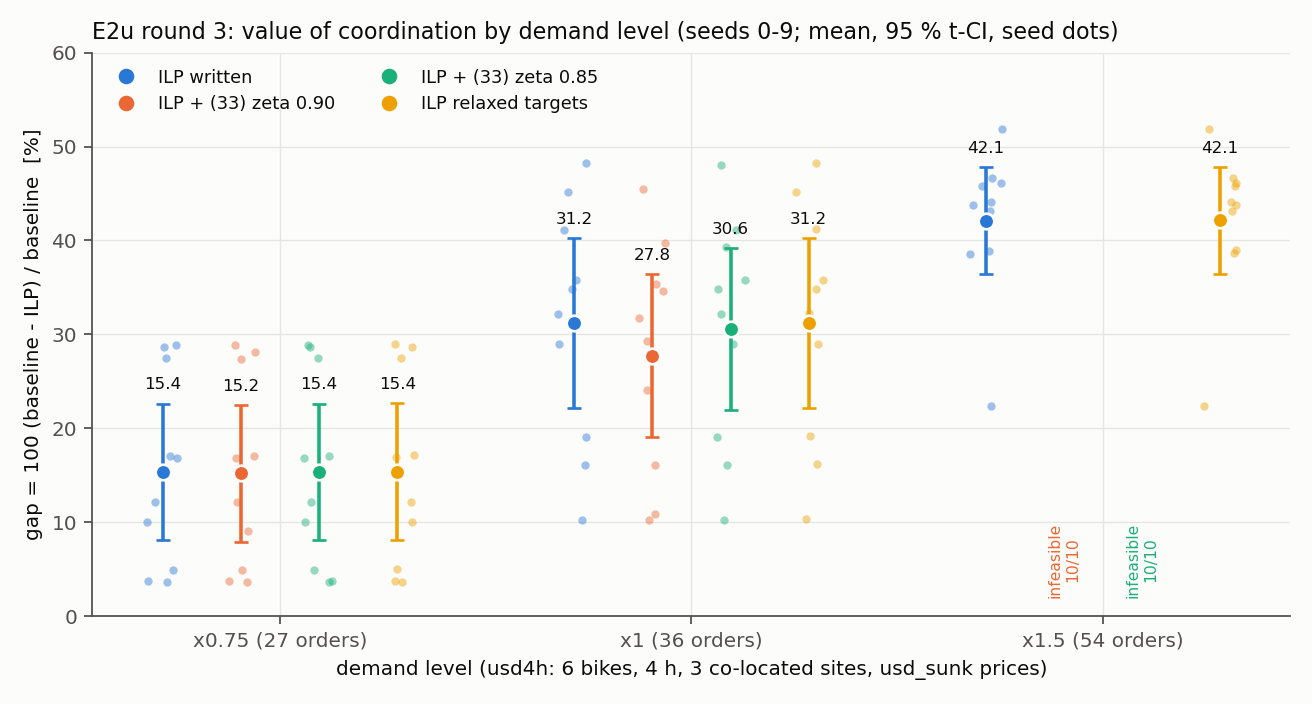
\includegraphics[width=\linewidth]{figs/e2_gap.png}
\captionof{figure}{\small E2u. Gap per demand level (dots $=$ seeds, bar $=$ mean, whisker $=$ 95\,\% interval) for the written plan, the plan with the 90\,\% / 85\,\% service rule and the plan without end-of-day targets.}
\end{minipage}\hfill
\begin{minipage}[c]{0.50\linewidth}
\takeaway{The plan is cheaper on every evening (3.7--51.8\,\%). The saving is punctuality: 1.2 late orders per normal evening versus 16.5 for the rule, same share of orders served (87.5 vs 87.2\,\%). The plan's cost barely varies between evenings (4--5\,\%); the rule's varies 15--22\,\%.}
\caveat{The plan knows all 36 orders at 17:00; the rule learns them as they arrive. Part of the 29.6\,\% is foresight, not coordination (Issue 1). On quiet evenings the plan drops slightly more orders than the rule (1.5 vs 0.9 of 27) because at 30 USD a drop is cheaper than a late delivery (Issue 5).}
\end{minipage}

\subsection*{Service-share constraint -- What does a service guarantee cost?}
\noindent\textit{Question:} if the plan must serve at least 90\,\% (or 85\,\%) of orders, how much more does it cost, and is it always possible?

% source: E2U "Service-share constraint (33)" table and x1.5 infeasibility table
\begin{center}\small
\begin{tabular}{@{}L{2.2cm}L{1.6cm}L{2.0cm}L{4.3cm}L{4.3cm}@{}}
\toprule
Minimum served & Demand & Possible? & Extra cost over the plain plan & Share served: rule / plan / plan $+$ guarantee \\
\midrule
90\,\% & $\times$0.75 & 10 of 10 & 0.9 USD (0.2\,\%), 3 of 10 evenings affected & 96.7 / 94.4 / 95.6\,\% \\
90\,\% & $\times$1 & 10 of 10 & 37.4 USD (5.5\,\%), 8 of 10 affected, 1.4--176 USD & 87.2 / 87.5 / 92.2\,\% \\
90\,\% & $\times$1.5 & \textbf{0 of 10} & -- (best possible share 74--80\,\% where proven, $\le 83\,\%$ by bound; 49 of 54 required) & 62.6 / 69.8 / -- \\
85\,\% & $\times$1 & 10 of 10 & 8.0 USD (1.1\,\%), 2 of 10 affected & 87.2 / 87.5 / 88.6\,\% \\
\bottomrule
\end{tabular}
\end{center}
\noindent\begin{minipage}[c]{0.47\linewidth}\centering
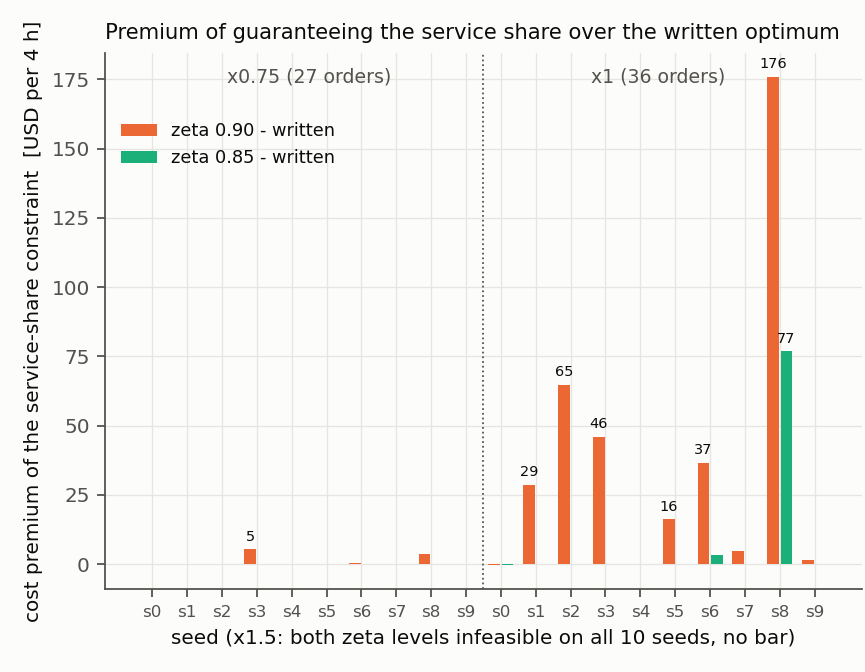
\includegraphics[width=\linewidth]{figs/e2_zeta_panel_a.png}
\captionof{figure}{\small Service share: extra cost of the 90\,\% / 85\,\% guarantee per seed (no bars at $\times$1.5: infeasible on all 10 seeds).}
\end{minipage}\hfill
\begin{minipage}[c]{0.50\linewidth}
\takeaway{A 90\,\% promise is almost free on a quiet evening, costs about 5\,\% on a normal one (bought with a few late deliveries: 5.7 instead of 1.2), and cannot be kept on a busy evening with 6 bikes: that is a fleet-size question, not a scheduling one (Issue 4).}
\caveat{The guaranteed plan still beats the rule by 27.8\,\% $\pm$ 8.7 at normal demand. The 1.5$\times$ infeasibility was proven by solver bounds on 4 of 10 seeds rather than closed solves; how many bikes would make 90\,\% feasible has not been run.}
\end{minipage}

\subsection*{E3u -- Are shuttles and separate charging hubs worth it?}
\noindent\textit{Question:} if charging moves to a separate hub (same 9 batteries and 6 chargers in every layout), what does it cost, and how much do shuttles help? (5 seeds, all 60 solver cells solved.)

% source: E3U "Headline numbers" and tables T1-T3, T5
\begin{center}\small
\begin{tabular}{@{}L{3.4cm}rrL{2.8cm}L{2.7cm}L{2.4cm}@{}}
\toprule
Layout & Plan, USD & No shuttles & Value of shuttles & Extra vs (a) & Gap vs rule \\
\midrule
(a) 3 sites swap $+$ charge & 638 & 638 & 0.01 & -- & 21.3 $\pm$ 11.3\,\% \\
(b) 3 swap sites $+$ 1 hub & 690 & 699 & 8.6 $\pm$ 10.1 (0 without targets) & $+$52.2 (29.2 is hub rent) & 18.4 $\pm$ 10.6\,\% \\
(c) 3 swap sites $+$ 2 hubs & 720 & 728 & 8.6 $\pm$ 10.1 (0 without targets) & $+$81.4 (58.4 is hub rent) & 17.8 $\pm$ 10.4\,\% \\
\bottomrule
\end{tabular}
\end{center}
\takeaway{Separating charging from swapping costs about 23 USD of operations plus the hub rent; the ranking co-located $<$ 1 hub $<$ 2 hubs holds on every seed. Shuttles are worth nothing once the end-of-day targets are dropped: in a 4 h window the 9 spares never run out (Issue 3). The rule's own ``ship when low'' habit hurts on every layout and every seed ($+$165 to $+$207 USD per evening: 5--14 trips at 20 USD each, at most one order rescued).}
\caveat{The ``shuttles allowed'' cells of layouts (b) and (c) stop where the solver could not prove the answer within 2\,\%, even with 600 s, so 8.6 USD is a lower bound (upper bound 22 USD; Issue 7). Intervals on the gap are wide ($\pm$ 10--11 points, 5 seeds).}

\subsection*{E4u -- How big should a station be?}
\noindent\textit{Question:} what happens to cost when spare batteries ($B$), chargers ($C$) and site power ($P$) change? (6 seeds for the battery sweep; 3 for chargers and power; full 20-cell $B \times C$ grid on seed 0.)

% source: E4U "Sweep B" tables (ILP and baseline), summary sentences 1-3
\begin{center}\small
\begin{tabular}{@{}L{3.2cm}rrL{6.6cm}@{}}
\toprule
Spares per site & Plan, USD & Rule, USD & Worth of the extra battery to the rule \\
\midrule
1 & 641 & 1,023 & 44.2 $\pm$ 21.6 USD per evening (1 $\to$ 2) \\
2 & 641 & 890 & 6.1 $\pm$ 10.8 (2 $\to$ 3), not significant \\
3 (default) & 641 & 872 & $\approx 0$ \\
4 & 642 & 874 & $\approx 0$ \\
6 & 644 & 867 & -- \\
Free sizing by the plan & \multicolumn{3}{L{10.7cm}}{buys only 3--4 batteries and 2--4 chargers for the whole area (default 9 and 6), saving 1.43 USD; at those lean sizes the rule collapses to 80\,\% served and the gap is 33.5\,\% $\pm$ 10.5} \\
\bottomrule
\end{tabular}
\end{center}
\noindent\begin{minipage}[c]{0.44\linewidth}\centering
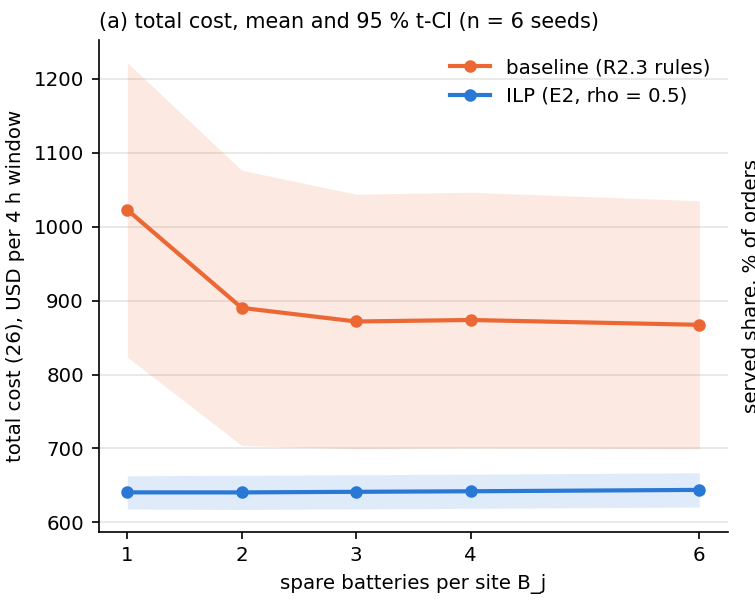
\includegraphics[width=\linewidth]{figs/e4_B_panel_a.png}
\captionof{figure}{\small E4u. Total cost against spare batteries per site, plan (blue) and rule (orange); band $=$ 95\,\% interval over 6 seeds.}
\end{minipage}\hfill
\begin{minipage}[c]{0.53\linewidth}
\takeaway{For the plan one spare per site is already enough (a second is worth 0.35 USD; chargers and power are worth exactly 0, shown by solves at every size). Station capital is the rule's lever, not the plan's; on 3 of 6 seeds the rule never reaches the plan's service level even with 6 spares per site.}
\caveat{The charger and power sweeps rest on 3 seeds (values flat to 0.1 USD; Issue 12). The annualised figure (64,600 USD per battery-year for the rule's first spare) assumes every 4 h window looks like the dinner peak; it is an upper-bound convention.}
\end{minipage}

\subsection*{E8 -- Does the advantage survive real Manhattan data?}
\noindent\textit{Question:} with real restaurants, real neighbourhood demand weights and real candidate sites in Midtown, is the plan still better? (6 riders, 36 orders, 10 seeds, two station placements.)

% source: E8 section 2 (headline table: price of (17)-(18) 0.28 +/- 0.06 busiest, 0.26 +/- 0.05 grid), section 2a, section 4 (decomposition), section 5 (siting)
\begin{center}\small
\begin{tabular}{@{}L{4.8cm}rrL{4.4cm}@{}}
\toprule
Station placement & Rule, USD & Plan, USD & Gap \\
\midrule
Busiest restaurant cells & 1,014 & 670 & \textbf{31.8\,\% $\pm$ 8.2} \\
Landmarks (8th Ave / W 34th, Union Sq, Grand Central) & 997 & 670 & 30.5\,\% $\pm$ 8.6 \\
Service (busiest) & \multicolumn{3}{L{9.5cm}}{plan 85.8\,\% served, 1.5 late, 0.83 h to the door, 95 km; rule 83.9\,\%, 17.8 late, 1.07 h, 110 km} \\
Where the saving is & \multicolumn{3}{L{9.5cm}}{59\,\% lateness, 35\,\% waiting, 6\,\% dropped; end-of-day targets cost 0.28 USD (busiest) / 0.26 USD (landmarks)} \\
\bottomrule
\end{tabular}
\end{center}
\noindent\begin{minipage}[c]{0.40\linewidth}\centering
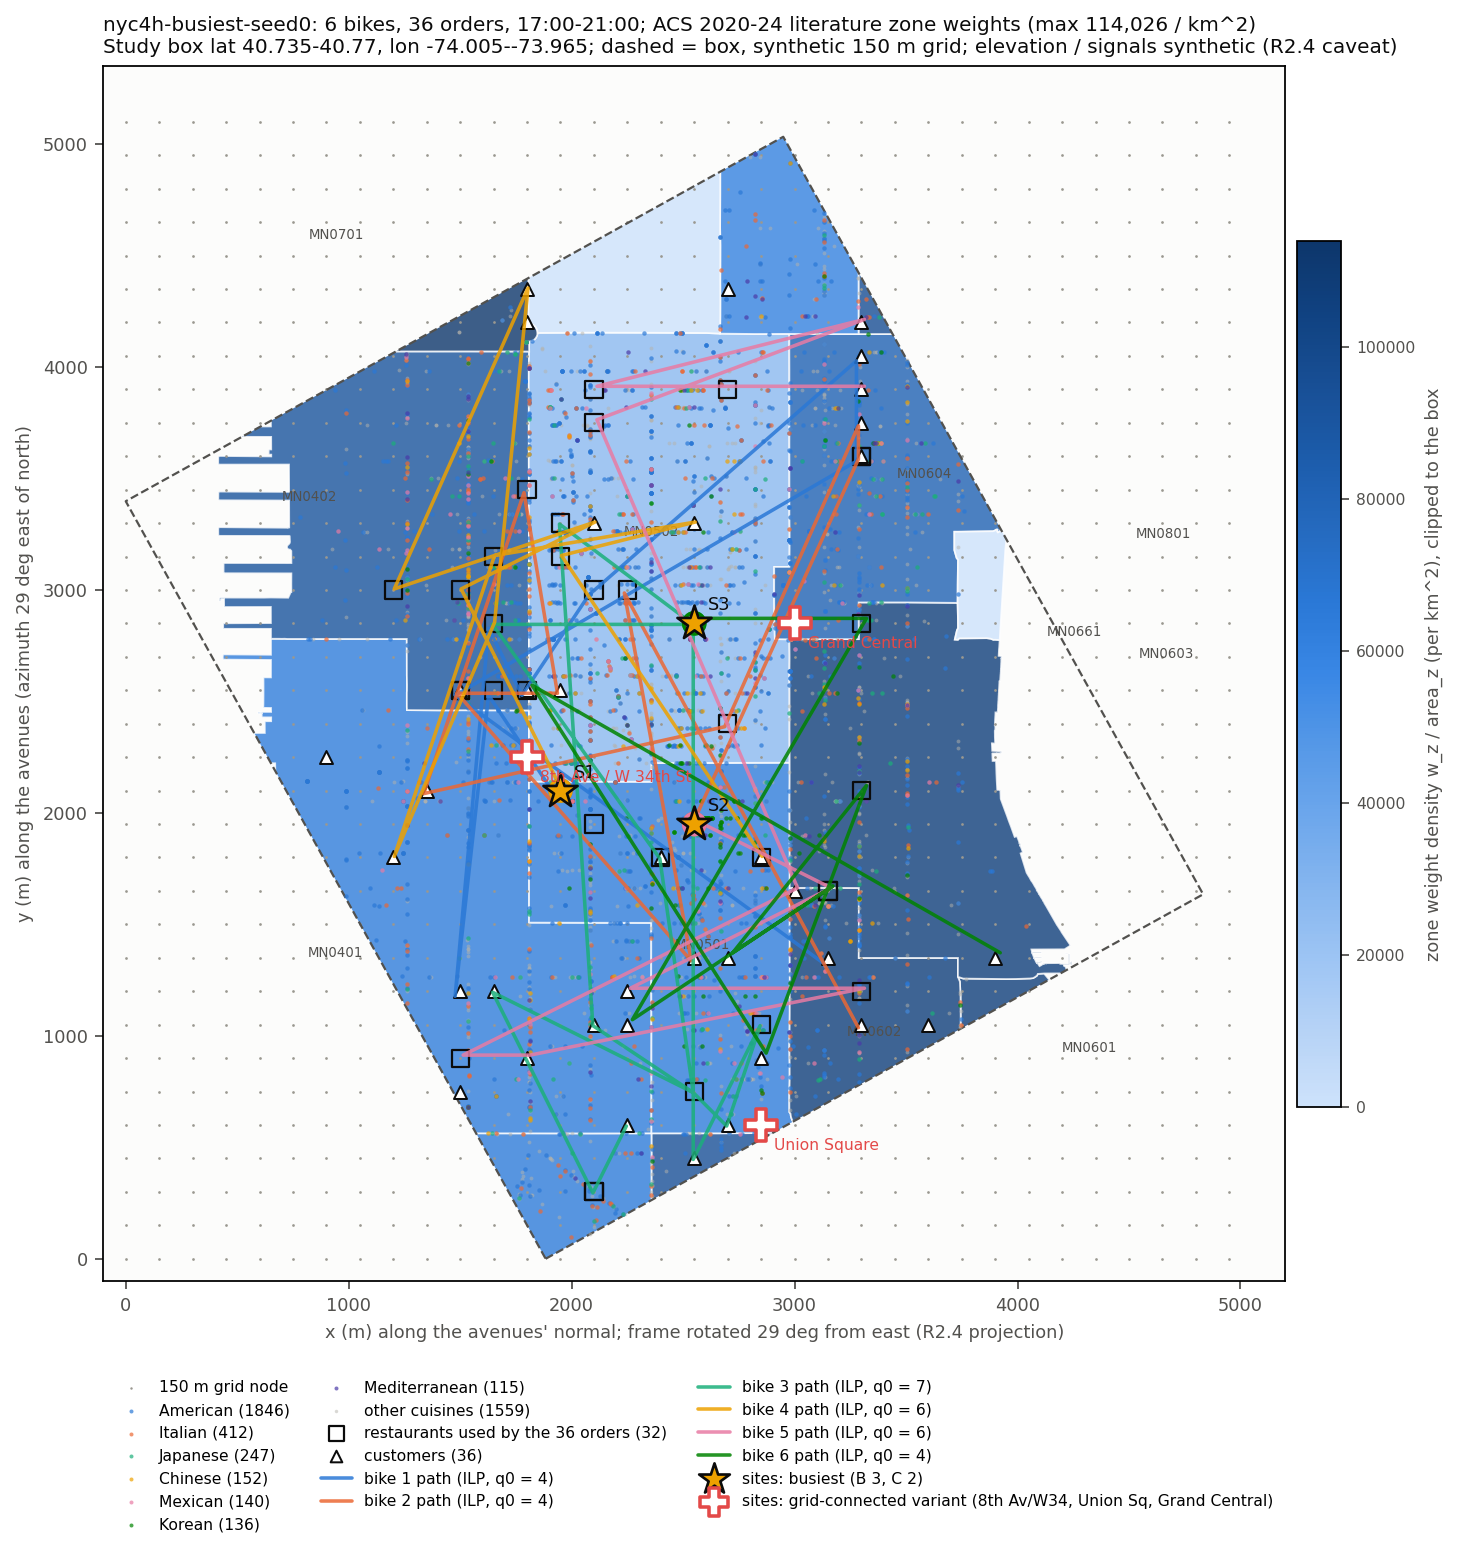
\includegraphics[width=\linewidth]{figs/e8_map.png}
\captionof{figure}{\small E8, seed 0. Study box with restaurants, neighbourhood demand heat map, both site placements (stars $=$ busiest cells, crosses $=$ landmarks) and the six rider paths.}
\end{minipage}\hfill
\begin{minipage}[c]{0.57\linewidth}
\takeaway{Yes: positive on all 20 instances (18--51\,\%), same shape as the synthetic evenings. The plan's cost moves by at most 0.41 USD when the sites are relocated; the rule's swings by $-9$ to $+6$\,\% with no consistent direction. The plan absorbs where the stations are; the rule does not.}
\caveat{The street network, hills and signals are still synthetic (real points snapped onto a 150 m grid; Issue 8). The plan's repositioning moves were restricted (not the rule's), so each gap is a lower bound; the lossless check has not been run (Issue 6). All 40 solves were proven optimal in 28--64 s.}
\end{minipage}

\newpage
\subsection*{E9 -- Where to put the stations (bi-level siting)}
% source: E9 = ebike_swap_sim/outputs/e9_bilevel/RESULTS_E9.md (sections 3.3, 3.5, 3.6, 3.7) and sweep/, deck/, access/, cross/ RESULTS_final.md
\noindent\textit{Question:} among 12 Midtown candidate corners, which stations should open, of which kind (swap-only, charge-only hub, or both) and how big, under an investment budget of $m \times 52{,}150$ USD, when the plan runs the evenings? (Planner above, E2 as written below on 3 demand scenarios; 6 bikes, 36 orders, start charge 3--6 of 12; cost per evening $=$ station cost spread over 4 h windows $+$ expected operating cost.)

\begin{center}\small
\begin{tabular}{@{}L{2.4cm}L{4.4cm}L{2.2cm}L{1.9cm}L{1.3cm}L{2.4cm}@{}}
\toprule
Budget $m$ (USD) & Chosen layout & Investment used & Cost per evening, USD & Served & Deck planner regret \\
\midrule
1 (52,150) & L02 swap $+$ charge, 3 spares, 2 chargers & 52,150 (100\,\%) & 654.38 & 85.2\,\% & 0.68 (0.10\,\%) \\
2 (104,300) & L02 swap $+$ charge, 4 spares, 2 chargers & 52,600 (50\,\%) & 654.53 & 85.2\,\% & 12.56 (1.92\,\%) \\
3 (156,450) & same & 52,600 (34\,\%) & 654.53 & 85.2\,\% & 25.53 (3.90\,\%) \\
4 (208,600) & same & 52,600 (25\,\%) & 654.53 & 85.2\,\% & 38.78 (5.93\,\%) \\
Any second site & \multicolumn{5}{L{13.8cm}}{$+$11.9 to $+$12.2 USD per evening for a swap-only or co-located site, $+$29.4 for a charge-only hub, against an operating saving of at most 1.09 USD; shuttles used in 0 of 84 solves; role sets \{SC\}, \{S, SC\}, \{S, C, SC\} give the identical answer} \\
Access rule (every zone within 1.8 km of a swap point) & L02 $+$ L05 (Rockefeller south) & 103,050 & 666.61 ($+$12.08) & 85.2\,\% & 11 of 11 zones covered \\
Cross-check, 5 seeds & \multicolumn{5}{L{13.8cm}}{location robust (L02 under the plan and under the rule; L01 a tie); size not: the 4th spare is worth 47.4 USD per evening to the rule and 0.15 USD to the plan} \\
\bottomrule
\end{tabular}
\end{center}
\noindent\begin{minipage}[c]{0.60\linewidth}\centering
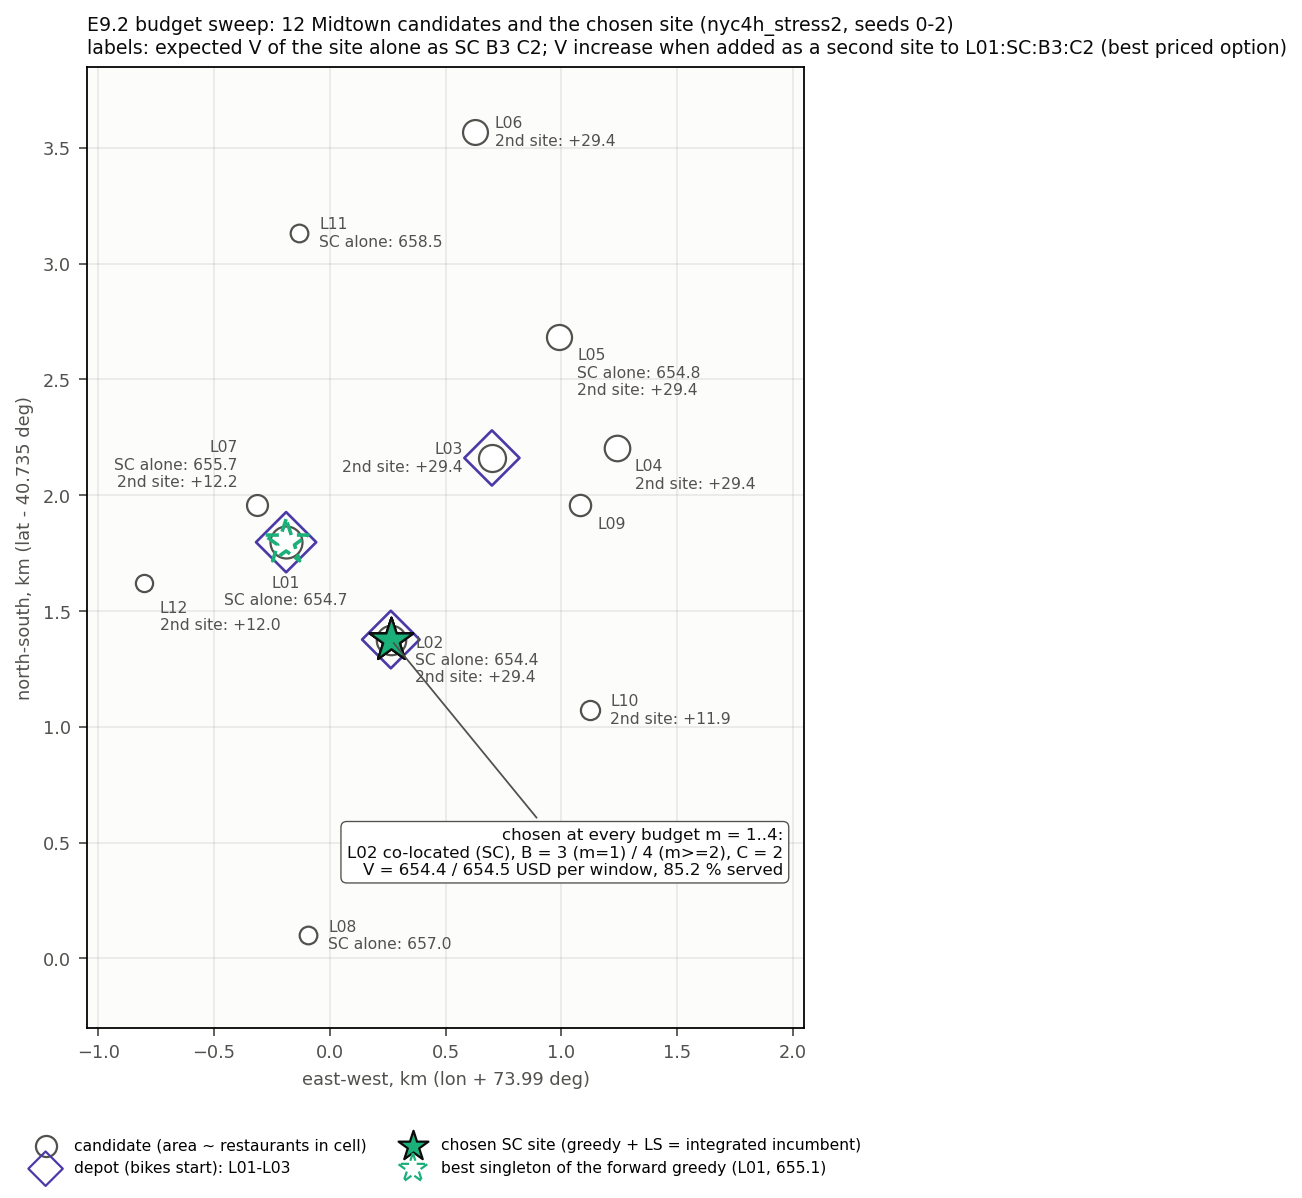
\includegraphics[width=\linewidth]{figs/e9_map_sites.png}
\captionof{figure}{\small E9. The 12 candidates (circle area $\sim$ restaurants in the cell), the chosen site L02 (star) and, per candidate, its cost per evening as the only site or the cost increase when added as a second site.}
\end{minipage}\hfill
\begin{minipage}[c]{0.37\linewidth}\raggedright
\takeaway{\textbf{One well-stocked swap-and-charge station is the whole infrastructure: every method (exhaustive enumeration, integrated two-stage program, greedy $+$ local search, all three role sets) returns L02 alone, and the budget beyond one unit stays unspent. The proposal's rule ``one station per budget unit'' loses 0.1 / 1.9 / 3.9 / 5.9\,\% at $m = 1..4$, exactly the setup of the extra stations.}}
\caveat{With 6 bikes the fleet, not the batteries, limits service: the served share is 85.2\,\% for every layout with $\ge 3$ spares, so siting moves only travel and electricity (Issue 13); the 12-candidate answers are heuristic incumbents without a certified gap (Issue 14); the access run at 1.2 km was cut short (Issue 15). Same synthetic-grid caveat as E8.}
\end{minipage}

% ======================================================================
\section*{6. Problems and open issues}
% ======================================================================
% brief_issues.tex -- issue boxes for the supervisor brief (no preamble).
% Environments \begin{issuebox}{<title>} and \begin{notebox}{<title>} are defined by the assembler.
% Every number below is copied from a report; the source file is given in a LaTeX comment.
% Vocabulary: "plan" = E2 integer program, "rule" = baseline policy, "USD" after the number, "dropped" = unserved.
% Order: Issues 1-3 could change the headline; 4-6 limit what we can claim; 7-12 are housekeeping (one table).

\noindent\textbf{How to read:} Issues 1--3 could change the headline; Issues 4--6 limit what we can claim; Issues 7--12 are housekeeping (one table); Issues 13--15 concern the siting study (E9).

% ---------------------------------------------------------------------------
% 1. Foresight vs coordination
% source: notes/E2_formulation_review.md (SC-2); outputs/e2u_round3/RESULTS_final.md (gap tracks baseline lateness r = 0.91); outputs/e8_round3/RESULTS_final.md (r = 0.98)
\begin{issuebox}{Issue 1 -- The 29.6\,\% headline mixes coordination with perfect foresight}
\textbf{What we saw:} the plan knows all 36 orders at 17:00 (27--30 min before they are ready); the rule learns each order when it is placed. Evening by evening, the gap follows the rule's lateness (correlation 0.91 in E2u, 0.98 in E8).\\
\textbf{Why it matters:} we cannot say how much of 29.6\,\% $\pm$ 5.6 is \emph{planning together} and how much is \emph{knowing the future}.\\
\textbf{Status:} open.\\
\textbf{Next step:} rolling-horizon wrapper (no change to the equations) on the same 30 evenings with look-ahead 0 / 10 / 20 min; what survives at zero look-ahead is coordination proper.
\end{issuebox}

% ---------------------------------------------------------------------------
% 2. Battery side never binds
% source: outputs/e8_round3/RESULTS_final.md (anomaly 8, siting table); outputs/e4u_round3/RESULTS_final.md (sweeps C, P; summary sentence 2); notes/E2_formulation_review.md (SC-1)
\begin{issuebox}{Issue 2 -- Stations, chargers, grid and shuttles never bind at this scale}
\textbf{What we saw:} with the targets off the plan buys 0 kWh in 20 of 20 Midtown runs; a charger or a kW is worth 0 USD; moving the stations changes the plan's cost by at most 0.41 USD (0.06\,\%). Detail: peak draw 3.33 kW against a 6--8 kW limit; every spare beyond the second \emph{costs} 0.25--0.31 USD per evening.\\
\textbf{Why it matters:} three questions of the proposal (station queues, charging, swap-oriented dispatch) have no content on these instances; the whole gain is dispatch.\\
\textbf{Status:} limitation of the instance, not of the equations.\\
\textbf{Next step:} energy-stressed family (8 bikes, 48 orders, start charge 2--4 of 12, one spare and one charger per site, 1.4 kW per site), then 8 h windows. Success $=$ a battery constraint with a positive shadow price, or a spare worth more than its 0.332 USD holding cost.
\end{issuebox}

% ---------------------------------------------------------------------------
% 3. End-of-day targets manufacture the shuttle value
% source: outputs/e3u_round3/RESULTS_final.md (Summary, T1, T2); notes/E2_formulation_review.md (SC-4);
%         outputs/e2u_round3/RESULTS_final.md (targets cost 0.34 USD); outputs/e8_round3/RESULTS_final.md section 2 (0.28 +/- 0.06 busiest, 0.26 +/- 0.05 grid)
\begin{issuebox}{Issue 3 -- Shuttles are worth 8.6 USD only because of the end-of-day battery targets}
\textbf{What we saw:} value of shuttles in the separated layouts: 8.6 $\pm$ 10.1 USD with the targets as written, \textbf{0.00 USD on 15 of 15 pairs} with the targets off. Mechanism: the ``one full battery at closing'' target at a swap-only site caps swaps at 4 of 9; one 22 USD shuttle with 2 batteries restores 6 swaps. In co-located layouts the targets cost 0.34 USD (E2u) and 0.28 / 0.26 USD (E8, busiest / landmarks) per evening.\\
\textbf{Why it matters:} the only reason to ship batteries in a 4 h window is ``be tidy at closing time''; the written transfer result is housekeeping, not replenishment.\\
\textbf{Status:} parameter choice ($\rho$, $R_{\mathrm{end}}$ are data in E2) -- Decision 1 on page 1.\\
\textbf{Next step:} set $R_{\mathrm{end}} = 0$ at swap-only sites; report a $\rho \times R_{\mathrm{end}}$ sensitivity grid; use the targets-off control as the like-for-like headline and the written targets as ``price of recovery''.
\end{issuebox}

% ---------------------------------------------------------------------------
% 4. 90 % service infeasible at busy demand
% source: outputs/e2u_round3/RESULTS_final.md (x1.5 table, anomaly 3, solver statistics: 14 TIME_LIMIT without incumbent, 4 INFEASIBLE 175-248 s, max-service solves 129-300 s, 70.9 min; wall 263.2 min); notes/E2_formulation_review.md (B8)
\begin{issuebox}{Issue 4 -- A 90\,\% service promise is impossible on a busy evening with 6 bikes}
\textbf{What we saw:} at 54 orders the most any schedule can serve is 74--80\,\% (proven on 6 seeds; at most 83\,\% by bound on the rest) against 90\,\% (49 of 54) or 85\,\% (46) required: infeasible on 10 of 10 seeds at both levels. The cost-optimal plan drops 16.3 orders (30\,\%), the rule 20.2 (37\,\%). Detail: 18 of the 20 busy-evening service-rule cells cost 300--600 s each (14 hit the 300 s limit with no solution found, 4 were proven infeasible in 175--248 s, each followed by a 129--300 s max-service solve), about 2.5 h of the 4.4 h wall.\\
\textbf{Why it matters:} ``infeasible'' is a fleet-size answer, not a scheduling one, and we have no number for how many bikes would be needed.\\
\textbf{Status:} open.\\
\textbf{Next step:} fleet sweep 6--10 bikes at 1.5$\times$ demand with the 90\,\% rule, 10 seeds; solve ``most orders served'' first and skip the cells the bound already rules out.
\end{issuebox}

% ---------------------------------------------------------------------------
% 5. Drop penalty vs waiting cost
% source: notes/SUMMARY.md round 2, 2.1 (usd_A table: 85.2 / 86.1 / 83.3 % vs 5.6 / 11.1 / 35.2 %); outputs/e2u_round3/RESULTS_final.md (anomaly 5: 8/30); outputs/e8_round3/RESULTS_final.md (anomaly 4: 5/20); notes/E2_formulation_review.md (SC-3)
\begin{issuebox}{Issue 5 -- The wage convention decides whether the plan drops orders; even now it drops more than the rule on 8 of 30 evenings}
\textbf{What we saw:} with rider wages inside the waiting price (variant \texttt{usd\_A}, 40 USD/h) the plan drops 83--86\,\% of orders against 6--35\,\% for the rule, because serving an ordinary order then costs about 31 USD, more than the 30 USD drop penalty. Under the default \texttt{usd\_sunk} (18 USD/h) the plan still drops more than the rule on 8 of 30 E2u and 5 of 20 E8 evenings: waiting is charged from order placement, so about 29 min of kitchen time (about 8.8 USD) that no schedule can shorten is priced.\\
\textbf{Why it matters:} the serve / drop margin is set by an accounting convention; readers will see ``the optimiser drops orders'' as a failure.\\
\textbf{Status:} parameter choice, no equation changes -- Decision 3 on page 1.\\
\textbf{Next step:} start charging waiting time from when the food is ready, not from when the order is placed (equivalent to raising the drop penalty by the kitchen wait); re-run E2u at normal demand and report the headline under both conventions; keep rider labour sunk and say so.
\end{issuebox}

% ---------------------------------------------------------------------------
% 6. NYC pruning restricts only the plan
% source: outputs/e8_round3/RESULTS_final.md (pruning caveat, Section 10); notes/workflow6_round2_review.json (revFair F2); notes/E2_formulation_review.md (SC-5)
\begin{issuebox}{Issue 6 -- The Midtown gap (31.8\,\%) is a lower bound: the pruning ties the plan's hands, not the rule's}
\textbf{What we saw:} to keep the Midtown model solvable the plan may reposition only into the 3 station nodes (0.55 M arcs instead of about 36 M). The rule never repositions elsewhere anyway, so it loses nothing; the plan loses pre-positioning towards restaurants.\\
\textbf{Why it matters:} the E8 number cannot be quoted as exact; the loss has never been measured.\\
\textbf{Status:} open (declared in the report, not resolved).\\
\textbf{Next step:} run the lossless variant on one seed; on the synthetic family the lossless pruning gave identical optima (615.15 / 659.60 USD) with 40\,\% fewer arcs.
\end{issuebox}

% ---------------------------------------------------------------------------
% 13-15. Siting study (E9)
% source: outputs/e9_bilevel/RESULTS_E9.md section 5 (items 1, 2, 3, 4, 6); cross/ and sweep/ RESULTS_final.md; access/RESULTS_final.md; validate/RESULTS_final.md
\begin{issuebox}{Issue 13 -- In the siting study the fleet binds, not the batteries}
\textbf{What we saw:} under the plan the served share is 85.2\,\% (85.6\,\% on five seeds), lateness 1.7--1.8 orders and the dropped-order penalty 160 USD for \emph{every} layout with at least three spares, from one site to four; siting and sizing move only riding (11.8--12.4 USD) and electricity (0--0.8 USD).\\
\textbf{Why it matters:} the stressed family makes station placement matter for the rule but still not for the plan, so the planner learns little beyond ``one site with three or more spares''; the siting question is answered, but on a family where it is nearly degenerate.\\
\textbf{Status:} open.\\
\textbf{Next step:} a deeper energy-stressed family (more bikes per site, lower start charge, longer window, or fewer spares per site, since 2 spares is the only size at which the plan reacts) and the same sweep there.
\end{issuebox}

\begin{issuebox}{Issue 14 -- The siting answers are heuristic incumbents without a certified gap}
\textbf{What we saw:} the integrated two-stage program on 12 candidates $\times$ 3 scenarios (5.35 M variables) returned only its warm start and no usable bound in 600 s; the only exact check is the small validation protocol (4 candidates, 2 seeds, $\le 2$ spares), where exhaustive enumeration and the integrated program agree on L02 at 676.22 USD (bound 668.04, gap 1.21\,\%). That validation layout (2 spares, 1 charger) is the worst of the seven chosen layouts on the full menu ($+$8.3 USD under the plan, $+$150.6 USD under the rule).\\
\textbf{Why it matters:} ``one site is optimal'' rests on the exhaustive pricing of every single-site move and on the small-scale agreement, not on a proven bound; the validation certifies the machinery, not the number.\\
\textbf{Status:} open; acceptable for this brief with the caveat stated.\\
\textbf{Next step:} longer integrated runs (1,800 s or more) or a decomposition bound; quote the validation layout only as a protocol check, never as the optimum.
\end{issuebox}

\begin{issuebox}{Issue 15 -- Two search artefacts and a truncated access run (none changes a conclusion)}
\textbf{What we saw:} (i) the $m \ge 2$ answer (4 spares) lies outside the forward size menu ($\le 3$ spares) because the local search's size move is bounded only by the shelf ($K = 8$), and its value (654.53) is 0.15 USD \emph{worse} than the $m = 1$ layout (654.38), which is feasible at every budget: each budget restarted its search from the forward frontier and hit the 3-pass limit. (ii) With the access rule at 1.2 km the 120 min wall budget expired inside the second repair round: the three-site layout reported there ($+$24.4 USD) is the first usable covering layout, not the best, and one zone (MN0801) cannot be covered at 1.2 km by any candidate.\\
\textbf{Why it matters:} the per-budget values are not monotone and an enumeration restricted to the menu cannot return the chosen layout (effects 0.15--0.45 USD against 12--39 USD differences); only the 1.8 km access numbers ($+$12.08 USD, 11 of 11 zones) should be quoted.\\
\textbf{Status:} known, not fixed in this run.\\
\textbf{Next step:} seed budget $m$ with the results of all lower budgets, let the local search exhaust its passes, align the size move with the menu; price L02 $+$ L05 $+$ L06 and L02 $+$ L06 $+$ L08 directly (6 solves) and run the integrated program with the access rows at 1.8 km, $m = 2$.
\end{issuebox}

% ---------------------------------------------------------------------------
% 7-12. Smaller limitations, one table
% source: 7  outputs/e3u_round3/RESULTS_final.md (T8, anomaly 10: 10 cells, gap 1.79-2.00 %, 600 s; interval [8.6, 22.2] USD)
%         8  outputs/e8_round3/RESULTS_final.md (geometry caveat, Section 6: 1.80 vs 1.86 km); README.md Section 7
%         9  notes/cost_calibration.md (Section 0 table: F_j 4.0-29.0 base 12.0 low; v_i 40-120 $/h); E3U (hub rent 56-72 % of separation cost)
%         10 notes/SUMMARY.md round 2, 1.5 and 4.9 (26.1 % of 4,607 restaurants unreachable; 8.9 % if cafes -> American); notes/literature_demand_model.md Section 6; notes/datasets.md
%         11 notes/E2_formulation_review.md (B5); notes/SUMMARY.md round 1, 4.6 (64.4 vs 27.8 levels, 6.6 swaps; seed 0 615.146 vs 615.362)
%         12 outputs/e2u_round3/RESULTS_final.md (seeds 5-9: 21.9 -> 29.6 %, rule 1311 vs 1022 USD, plan 765 vs 727 USD, CV 4-5 % vs 15-22 %); outputs/e4u_round3/RESULTS_final.md (anomaly 8, C / P sweeps n = 3)
%         (12, for the record: the script figures use z = 1.96, the reports exact t, +/- 5.38 vs +/- 5.61 on the headline; means identical)
\begin{center}\small
\begin{tabular}{@{}L{2.4cm}L{7.6cm}L{4.6cm}@{}}
\multicolumn{3}{@{}l}{\normalsize\textbf{Smaller limitations (Issues 7--12).}}\\[2pt]
\toprule
Issue & What & Next step \\
\midrule
7 -- Solver gap & 10 E3u cells (separated layout, shuttles allowed) stop where the solver could not prove the answer within 2\,\%, even with 600 s; the shuttle value is an interval 8.6--22.2 USD, and more seeds or minutes will not close it. & Setting $R_{\mathrm{end}} = 0$ at swap-only sites (Issue 3) removes the shuttle and closes these cells. \\
8 -- Synthetic geometry & Street network, hills and traffic lights are synthetic even in the Midtown instance (real points snapped to a rotated 150 m grid); mean trip 1.80 km vs 1.86 km synthetic. Real data change \emph{where} demand sits, not how far bikes ride. & Connect the city's street centrelines and elevation data to the route library (interface exists). \\
9 -- Low-confidence prices & Station rent 4--29 USD per 4 h (base 12, confidence low), lateness price 40--120 USD/h, charger and shuttle prices low; hub rent is 56--72\,\% of the separation cost in E3u. & Run the low / high price envelopes already in \texttt{cost\_calibration} as a sensitivity. \\
10 -- Demand inputs partly assumed & 26.1\,\% of the 4,607 restaurants fall in a cuisine class that is never sampled (cafes, bakeries, desserts); the hourly curve (dinner 45\,\%, lunch 28\,\%, late 12\,\%) is an assumption; the Kaggle order file has no timestamps or coordinates. & Map cafes to ``American'' (unreachable share drops to 8.9\,\%); digitise the city's 2022 hourly delivery-trip chart. \\
11 -- Energy rounding & Each leg is rounded up to a whole 50 Wh level, so the plan uses 64.4 levels per Midtown evening against 27.8 physical (2.3$\times$) and riders swap about 6.6 times instead of 2--3; the headline gap is unaffected (seed 0 moves 0.2 USD). & Re-run with 25 Wh levels (24 per battery) or whole-route rounding; report swaps under both. \\
12 -- Wide intervals, few seeds & Intervals are wide because the rule's cost varies 4$\times$ more than the plan's (15--22\,\% vs 4--5\,\% between evenings); seeds 5--9 lifted the E2u gap from 21.9 to 29.6\,\% on the rule's side alone (rule 1,311 vs 1,022 USD, plan 765 vs 727 USD); charger / power sweeps rest on 3 seeds. & Charger / power sweeps on seeds 3--5 (cheap); quote per-level gaps where seeds differ; one interval convention everywhere. \\
\bottomrule
\end{tabular}
\end{center}

% ---------------------------------------------------------------------------
% Fixed items -- compact list
% source: notes/SUMMARY.md (round 1 code review: dominance pruning picked a farther bike 23 % of the time, battery dead zone; round 2, 1.6 fairness F1; round 3, 1.1);
%         outputs/e3u_round3/RESULTS_final.md (15 of 36 cells skipped in round 2, 0 SKIPPED_BUDGET now); outputs/e4u_round3/RESULTS_final.md ("Records used": P sweep 9 + 12 off-line B x C + skipped seed-2 B3_C4_P4 = 22)
%         (other fixes, for the record only: NYC time-profile ramp (E8 re-run); service-first variant replaced by the hard rule (33); E3u --analyse NaN crash; E4u pooled charger figure; E8 template text)
\begin{notebox}{Already fixed during rounds 1--3 (not open; listed for the record)}
\begin{itemize}\setlength{\itemsep}{1pt}
  \item \textbf{Rule fairness (round 1):} a pruning meant for the plan made the rule pick a farther bike 23\,\% of the time, and a ``battery dead zone'' left refused riders without a swap trip; both fixed.
  \item \textbf{Targets-off control (round 2):} the ``targets off'' copy silently changed the rule's charging reserve; fixed, and the rule's written and relaxed rows are now identical on 60 of 60 E3u rows and 20 of 20 E8 runs.
  \item \textbf{First siting launch (E9, superseded):} on an 8-bike family two searches reported ``no feasible layout'' (a wall-clock exhaustion was mapped to an infinite value; the access rule was enforced on single sites that can never cover all zones) and the budget sweep chose a one-spare swap-only site serving 7\,\% of orders (the cheap rule-based screen let only such sites through, with no served-share guard). Fixed in the relaunch (6-bike family, admissibility rule for swap-only sites, best-single-site start with a 50\,\% served-share guard, every evaluator failure reported as a status, access as repair-and-report); the archived numbers in \texttt{\_first\_attempt/} must not be quoted. Lesson: a cheap screening policy that values facilities differently from the plan can steer the search.
  \item \textbf{Skipped cells (round 2 $\to$ 3):} 15 of 36 E3u and 22 E4u cells (power sweep, 12 battery $\times$ charger cells, one skipped cell) were unsolved for wall-clock reasons; all solved in round 3, round-2 numbers reproduced exactly. Smaller fixes (demand ramp, report plumbing) are listed in \texttt{notes/SUMMARY.md}.
\end{itemize}
\end{notebox}


% ======================================================================
\section*{7. Next steps}
% ======================================================================
% source: REVIEW sections 5-7 (SC-1, SC-2, B12); SUMMARY round 3 sections 4-5; notes/bilevel_siting_design.md
\begin{itemize}\setlength{\itemsep}{2pt}
  \item \textbf{Energy-stressed instance family} (review item SC-1; answers Issues 2 and 4): 8 bikes, 48 orders, start charge 2--4 of 12, 1 spare and 1 charger per site at 1.4 kW, grid 4 kW; then an 8 h window. Success $=$ a battery constraint binds and a spare is worth more than its 0.332 USD holding cost. Includes a fleet-size sweep (6--10 bikes) at 1.5$\times$ demand: ``impossible with 6 bikes'' becomes a capacity curve.
  \item \textbf{Rolling horizon} (SC-2; answers Issue 1): re-solve the unchanged E2 every few steps on the orders known so far (look-ahead 0 / 10 / 20 min), carry rider and station state forward, price the whole evening afterwards. The share of the 29.6\,\% that survives at zero look-ahead is coordination proper. Each window solves in seconds.
  \item \textbf{Bi-level siting: done} (E9, Section 5; Issues 13--15). The planner (sites, roles, sizes under a budget of 52,150 USD per unit) with E2 as written below, run on the stressed Midtown family: one co-located station at L02 at every budget. Next: a family in which a second site changes who gets served (lower start charge, longer window or fewer spares per site, since 2 spares is the only size the plan reacts to); candidates across all of Manhattan; a multi-day lower level where chargers and hubs can matter; siting evaluated under the policy that will actually run the fleet.
\end{itemize}

% ======================================================================
\section*{8. Where to find things}
% ======================================================================
% source: README section 2 (repository table) and SUMMARY round 3 section 6
\noindent GitHub: \url{https://github.com/yuanmingchen922/Ebike_battey_swap} (English only; the supervisor's PDFs, instance dumps and workflow logs are not included). Paths relative to the repository root:
\begin{itemize}\setlength{\itemsep}{0pt}
  \item \texttt{README.md} -- overview, glossary, final numbers, how to run.
  \item \path{notes/} -- \path{SUMMARY.md} (full story of rounds 1--3), \path{DECISIONS.md} (every modelling choice), \path{E2_formulation_review.md} (the 32-proposal audit), \path{cost_calibration.md} (every USD figure with its range), \path{datasets.md}.
  \item \path{ebike_swap_sim/experiments/*_round3.py} -- one script per final experiment (code, baseline, generator and NYC loader one level up; 136 tests).
  \item \path{ebike_swap_sim/outputs/*_round3/RESULTS_final.md} (and \path{e1/RESULTS.md}) -- \textbf{the deliverables:} final reports, figures, raw records.
  \item \path{ebike_swap_sim/outputs/e9_bilevel/RESULTS_E9.md} -- the siting study, with sub-reports and figures in \path{validate/}, \path{sweep/}, \path{roles/}, \path{deck/}, \path{access/}, \path{cross/}; design in \path{notes/bilevel_siting_design.md}.
\end{itemize}


\end{document}
